يوضح المخطط التالي آلية كاملة لعمل المشروع. نبدأ من عرض البينة البرمحية الموجودة على الحاسوب المركزي والتي تتكون من نظام تشغيل روس مكون من ثلاثة عقد تتصل مع بعضها بتقنية \textenglish{Publish / Subscribe}، ثم نوضح تواصل هذه النظام مع مخدم بروتوكول MQTT المسؤول عن تحقيق التواصل مع الروبوتات حيث تشترك الربوتات بـ topic التي تحوي الرسائل الحاملة لنقاط المسار. بالنسبة للنظام البرمجي الموجود على كل من الروبوتات، تستقبل شريحة الاتصال الرسالة من المخدم وتنقلها إلى المعالج ليثيوم باتباعها وفق خوارزمية التصحيح. أنظر الشكل \ref{fig:08-graph}.


\begin{figure}
	\centering
	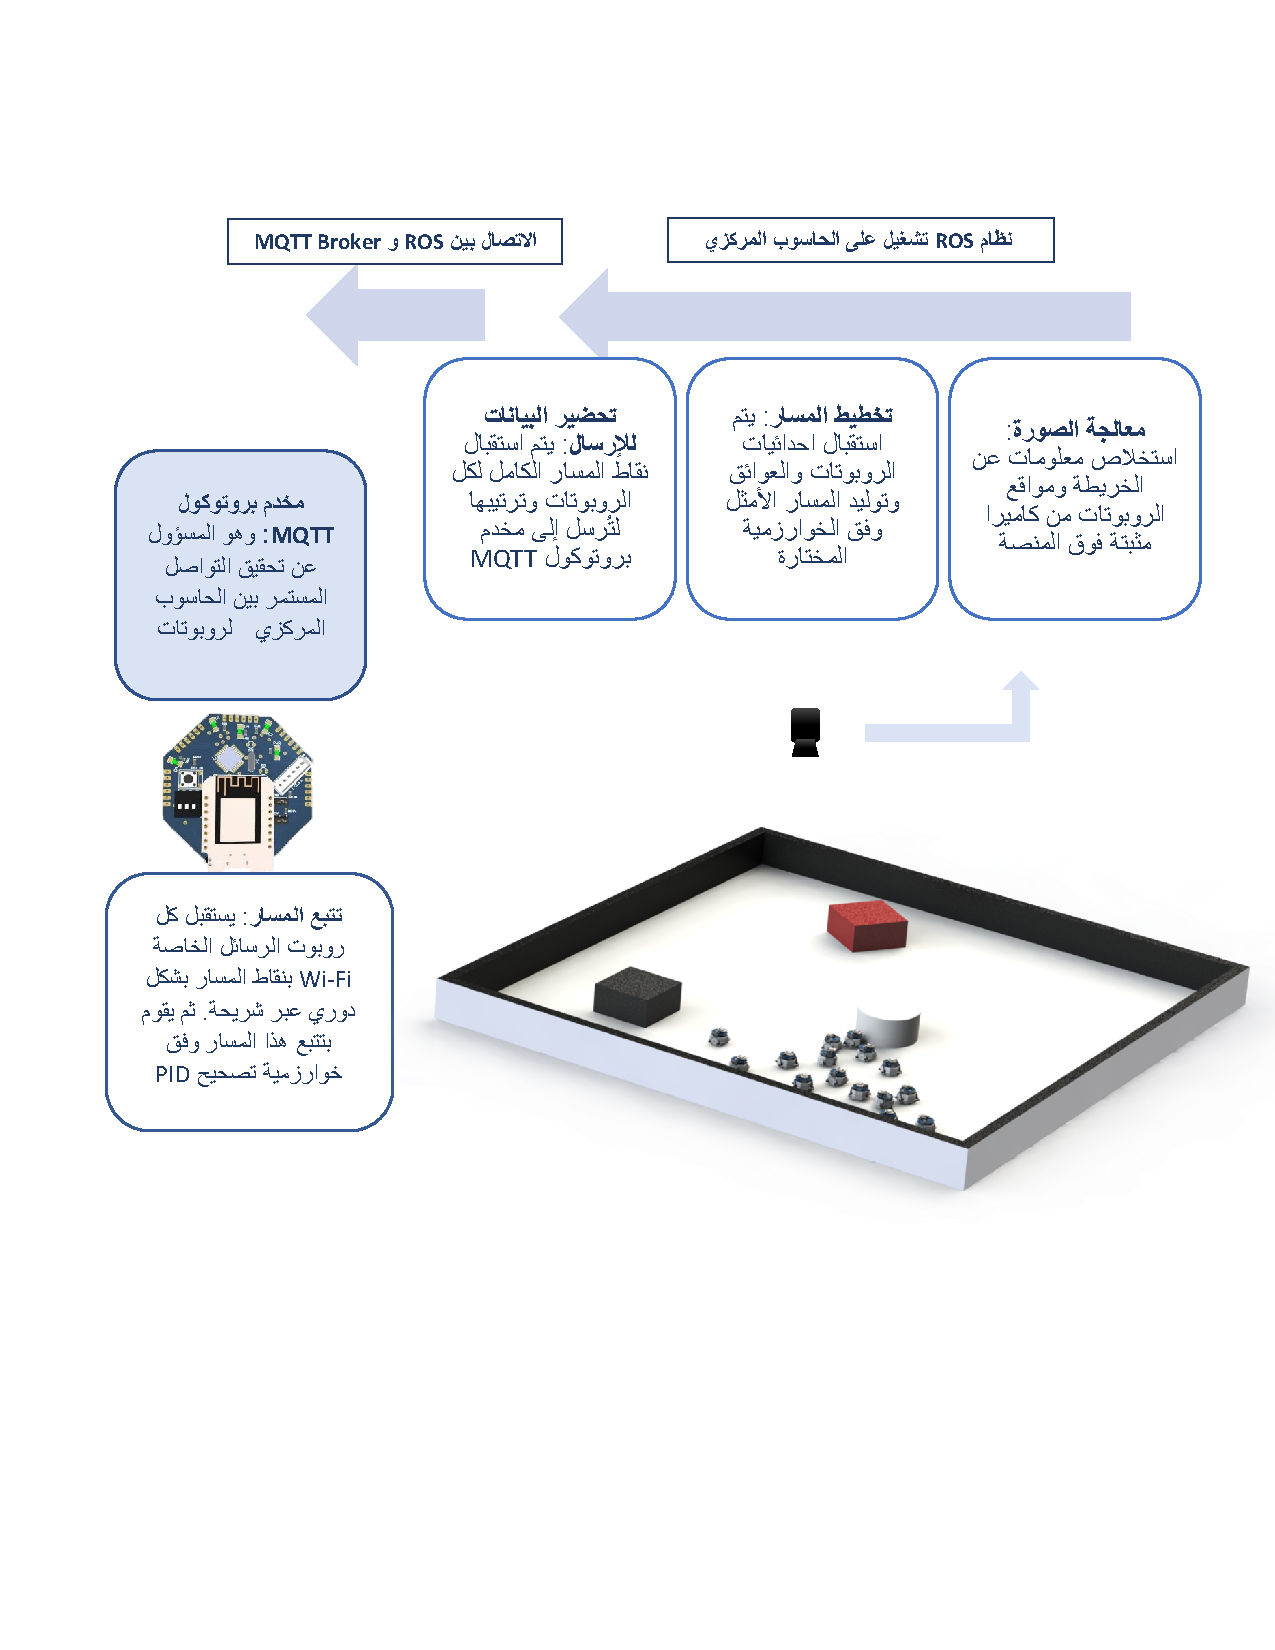
\includegraphics[width=0.95\linewidth]{08-graph}
	\caption{}
	\label{fig:08-graph}
\end{figure}
